%%% File: ./inputs/parts/EMBODIED_COGNITION.tex

%%% %%%%%%%%%%%%%%%%%%%%%%%%%%%%%%%%%%%%%%%%%%%%%%%%%%%%%%%%%%%%%%%%%%%%%%%%%%%%

Embodied cognition is the theory that an organism's body shapes its understanding of the environment it inhabits and grounds its perception of and interaction with that environment. Importantly, the environment completes a loop that links perception and action enabling the organism to formulate and test predictive models that guide behavior. Such models serve as the foundation for commonsense reasoning and provide a starting point for understanding a much wider range of concrete and abstract systems, giving rise to a tendency in humans to attribute self-styled agency to both animate and inanimate objects.

To ground our discussion, we consider a personal assistant that works with a software engineer in the role of an apprentice learning on the job, as was common in the guilds and trade associations of medieval cities. The programmer's apprentice we imagine here is a novice programmer but has the intuitive skills of an idiot savant, given that the apprentice has a suite of powerful programming tools as an integral part of its brain. These tools constitute the assistant's body, its peripheral nervous system if you will.

The original programmer's apprentice was the name of project initiated at MIT by Chuck Rich and Dick Waters and Howie Shrobe to build an intelligent assistant that would help a programmer to write, debug and evolve software. Our version of the programmer's apprentice is implemented as an instance of a hierarchical neural network architecture. It has a variety of conventional inputs including speech, text and vision, as well as output modalities including the ability to run code and display program output and execution traces. 

The programmer's apprentice relies on multiple sources of input, including dialogue in the form of text utterances, visual information from an editor buffer shared by the programmer and apprentice and information from a fully {\it{instrumented integrated development environment}} (FIDE) designed for analyzing, writing and debugging code adapted to interface seamlessly with the apprentice as we might move our limbs or direct our gaze. As in case of the legs you were born with, the apprentice has to learn how to use its prosthetic extensions.

This input is processed by a collection of neural networks modeled after the primary sensory areas in the primate brain. The outputs of these networks feed into a hierarchy of additional networks corresponding to uni-modal secondary and multi-modal association areas that produce increasingly abstract representations as one ascends the hierarchy as illustrate in Figure~{\urlh{#fig_Posterior_Cortex_Semantic_Cloud_Memory}{\ref{fig_posterior}}}.
  
%%% %%%%%%%%%%%%%%%%%%%%%%%%%%%%%%%%%%%%%%%%%%%%%%%%%%%%%%%%%%%%%%%%%%%%%%%%%%%%

%%% Figure~{\urlh{#fig_Posterior_Cortex_Semantic_Cloud_Memory}{\ref{fig_posterior}}}
\begin{figure}
%
  \begin{center} 
%    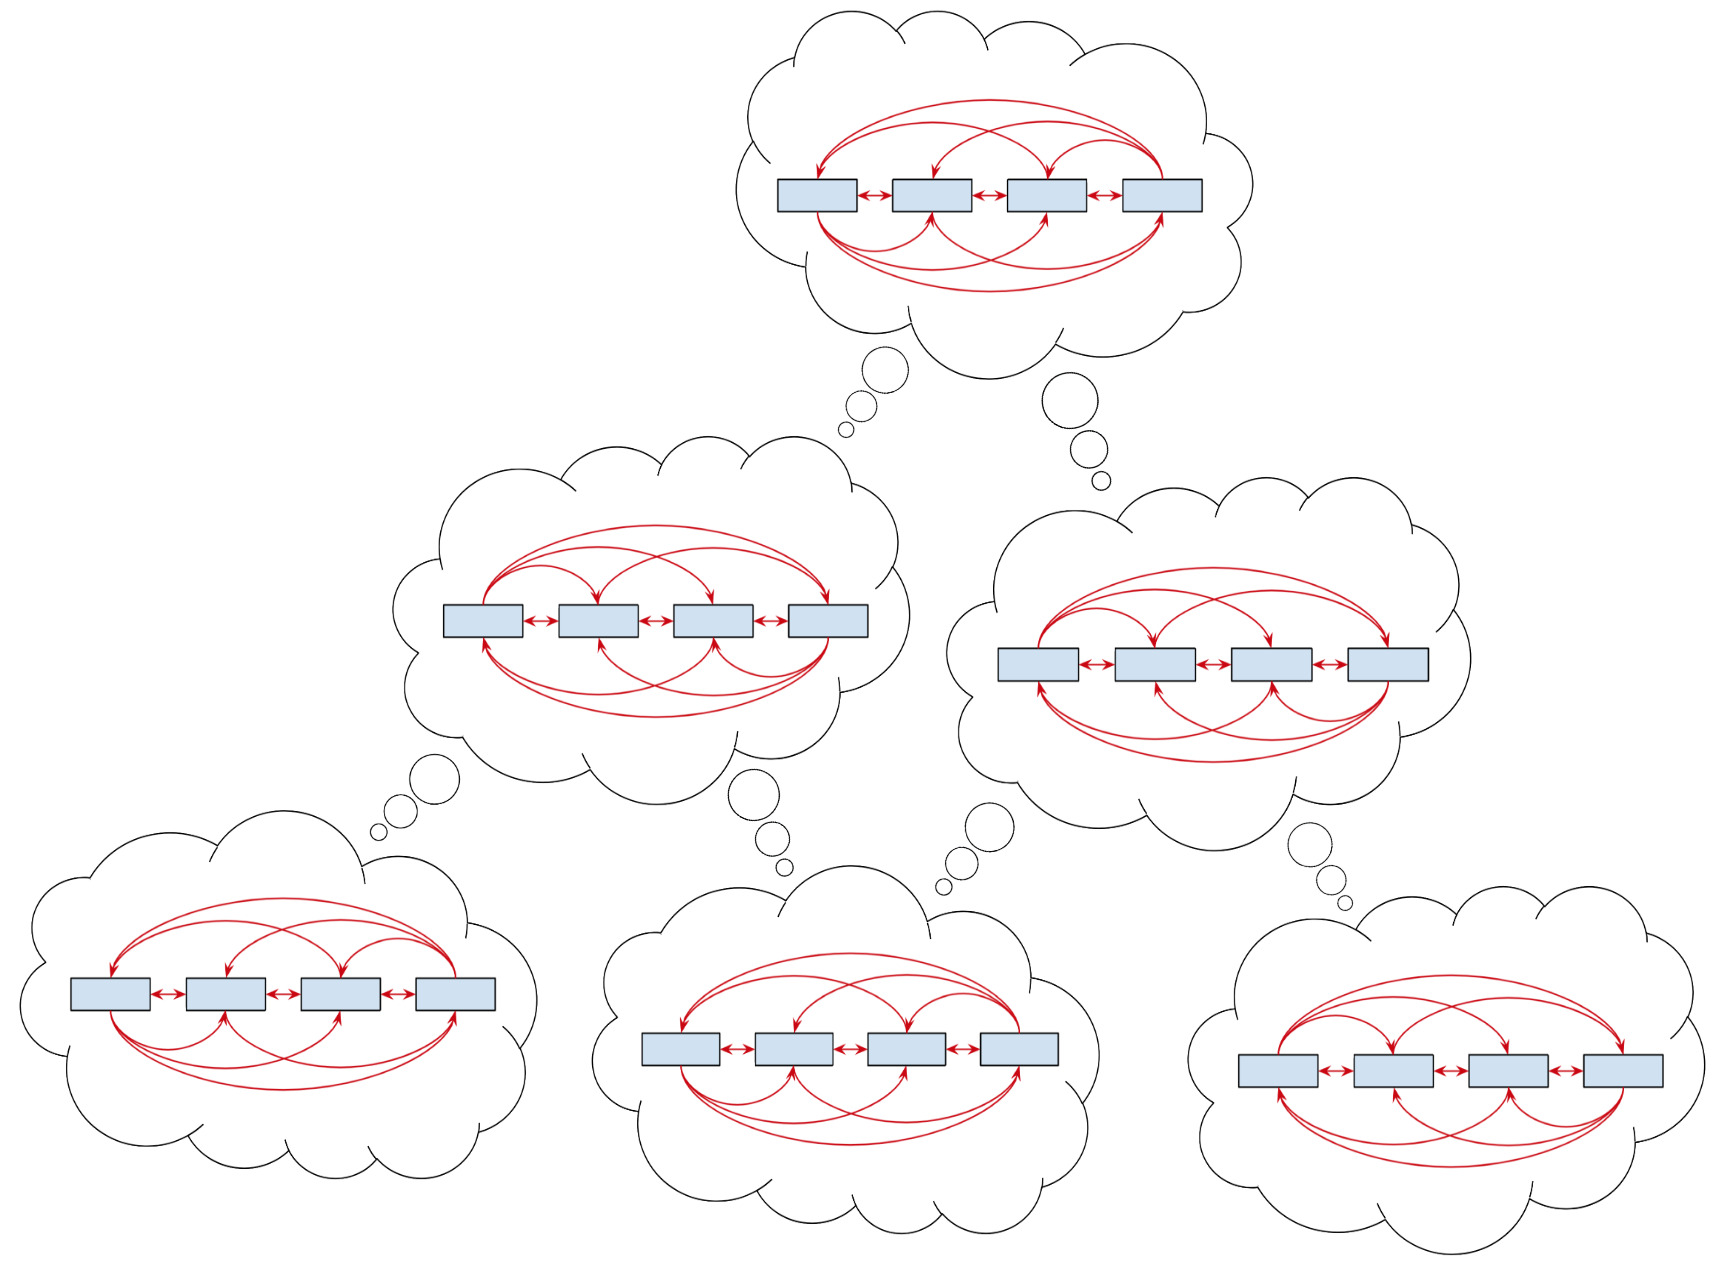
\includegraphics[width=400pt]{./figures/Posterior_Cortex_Semantic_Cloud_Memory.png} % 1106 × 973 pixels
    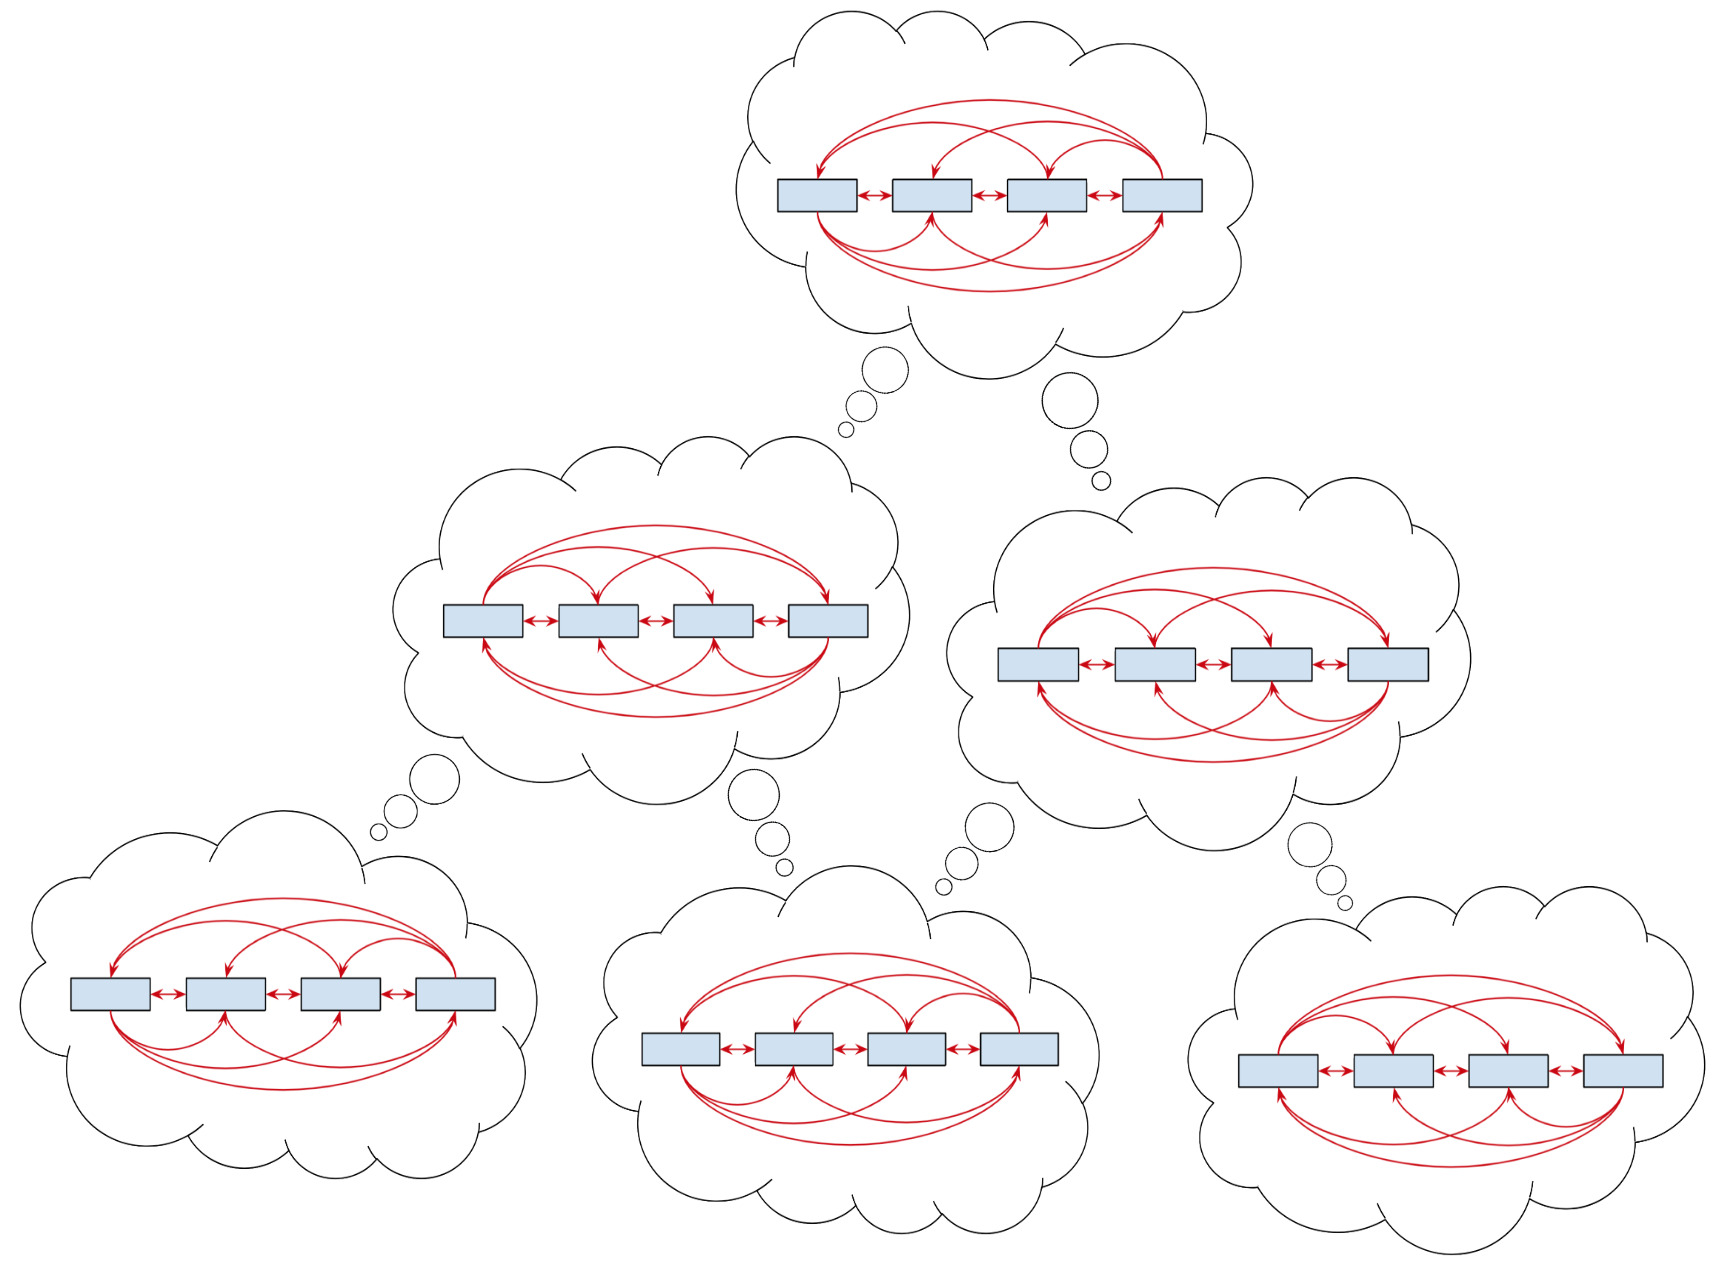
\includegraphics[width=200pt]{./figures/Posterior_Cortex_Semantic_Cloud_Memory.png} % 1106 × 973 pixels
  \end{center}
%
  \caption{The architecture of the apprentice sensory cortex including the layers corresponding to abstract, multi-modal representations handled by the association areas can be realized as a multi-layer hierarchical neural network model consisting of standard neural network components. This graphic depicts these components as encapsulated in thought bubbles of the sort often employed in cartoons to indicate what some cartoon character is thinking. Analogously, the technical term "thought vector" is used to refer to the activation state of the output layer of such a component. All of the bubbles appear to contain networks with exactly the same architecture, where one might expect sensory modality to dictate local architecture. The hierarchical architecture depicted here is modeled after the mammalian neocortex that appears to be tiled with columnar component networks called cortical columns that self-assemble into larger networks and adapt locally to accommodate their input. In practice, it may be necessary to engineer modality-specific networks for the lowest levels of the hierarchy \emdash{} analogous to the primary sensory and motor areas of the neocortex, but more general-purpose networks for the higher levels in the hierarchy \emdash{} analogous to the sensory and motor association areas.}
%
  \label{fig_posterior}
%
\end{figure}

%%% %%%%%%%%%%%%%%%%%%%%%%%%%%%%%%%%%%%%%%%%%%%%%%%%%%%%%%%%%%%%%%%%%%%%%%%%%%%%

Architecturally, the apprentice's FIDE is an instance of a differentiable neural computer (DNC) introduced by Alex Graves and his colleagues at DeepMind~\cite{GravesetalNATURE-16}. The assistant combined with its FIDE corresponds to a neural network that can read from and write to an external memory matrix, combining the characteristics of a random-access memory and set of memory-mapped device drivers and programmable interrupt controllers. The interface supports a fixed number of commands and channels that provide feedback.

The integrated development environment and its associated software engineering tools constitute an extension of the apprentice’s capabilities in much the same way that a piano or violin extends a musician. The extension becomes an integral part of the person possessing it and over time their brain creates a topographic map that facilitates interacting with the extension. We expect the same to occur in the case of the assistant. 

%%% %%%%%%%%%%%%%%%%%%%%%%%%%%%%%%%%%%%%%%%%%%%%%%%%%%%%%%%%%%%%%%%%%%%%%%%%%%%%
